\section{XoR}
\label{exo:XoR}
\begin{refsection}[exos/xor.bib]

keywords: model-based control; strength augmentation; hybrid actuation; pneumatic actuation; electric motors;\\

\begin{figure}[ht]
  \centering
  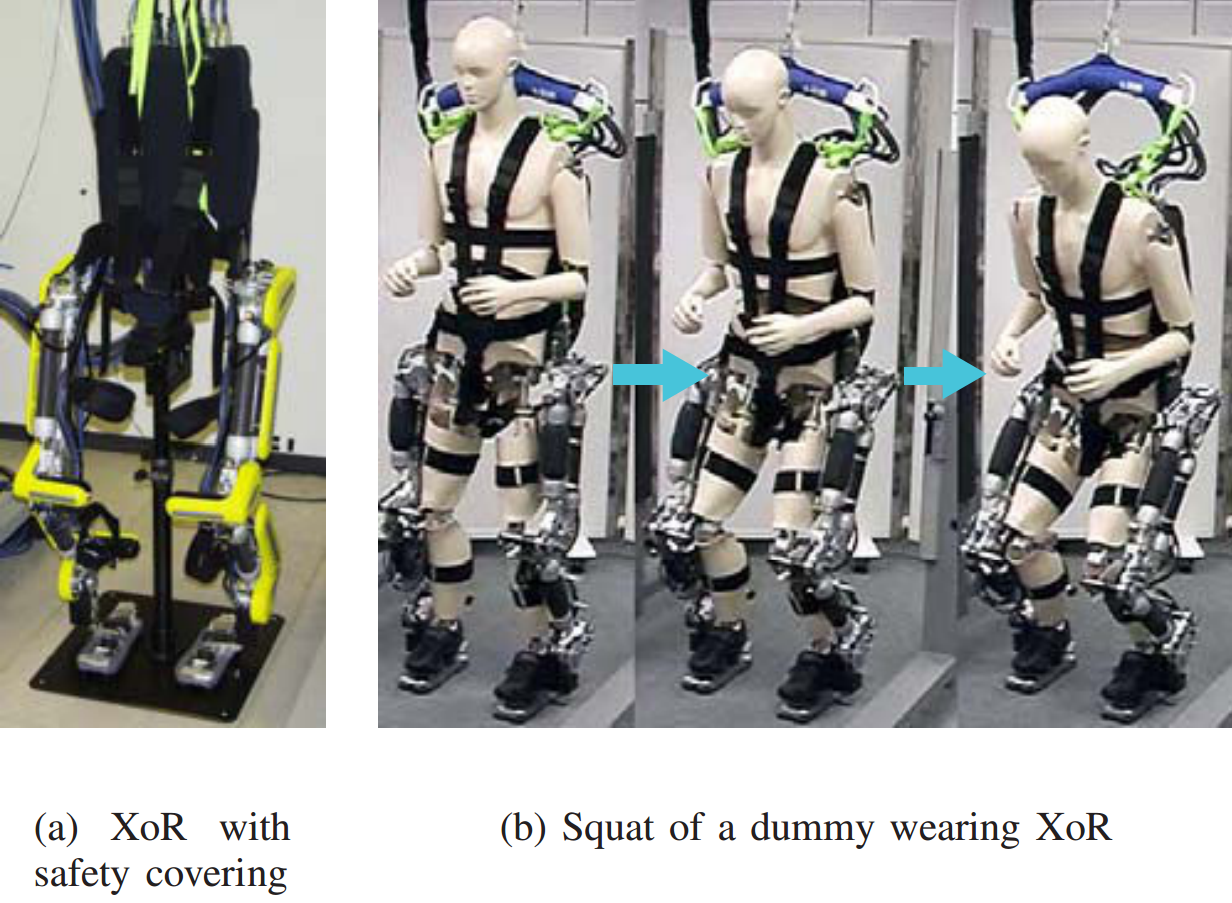
\includegraphics[width=4.0in]{exos/figs/xor.png}
\end{figure}

The XoR is a prototype light-weight, lower-body exoskeleton that uses a hybrid pneumatic-electric drive system that \textbf{reduces weight} while providing \textbf{precise torque control}, \textbf{backdrivability}, and a \textbf{desirable force / velocity} profile.  The exoskeleton is designed to serve in rehabilitation settings to augment operators' strength and assist with postural control for persons with disabilities.

\begin{figure}[ht]
  \centering
  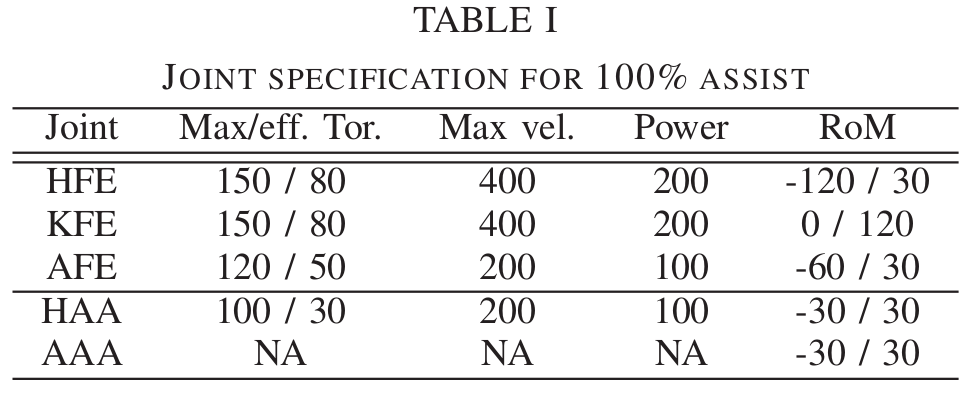
\includegraphics[width=3.5in]{exos/figs/xor_joint_rom.png}
\end{figure}

The XoR weighs 30kg and includes 10 DOF with 6 active joints (flexion / extension of hip, knee, and ankles) and 6 passive (hip abduction/adduction joints, hip rotation, and ankle adduction/abduction).  The active joints are powered by \textbf{hybrid actuators} comprised of an \textbf{air muscle} and an \textbf{electric motor}.  The hybrid actuation scheme uses a unilateral air muscle layout to compensate for gravity and bilateral electric motors with relatively small gear ratio (57.5) to serve as the dynamic compensator.

The actuation scheme is complementary in that the electric motors have a quick response time and produce high peak torque for short amounts of time, while air muscles have a delayed response (true of pneumatic systems in general due to the compressibility of air) with better power density and sustained torque.  The hybrid drive system sums the two to develop a desired torque profile that achieves the benefits of both and reduces weight and motor size.  The system offers high torque control with negligable stick-slip and backdrivability.

\begin{figure}[ht]
  \centering
  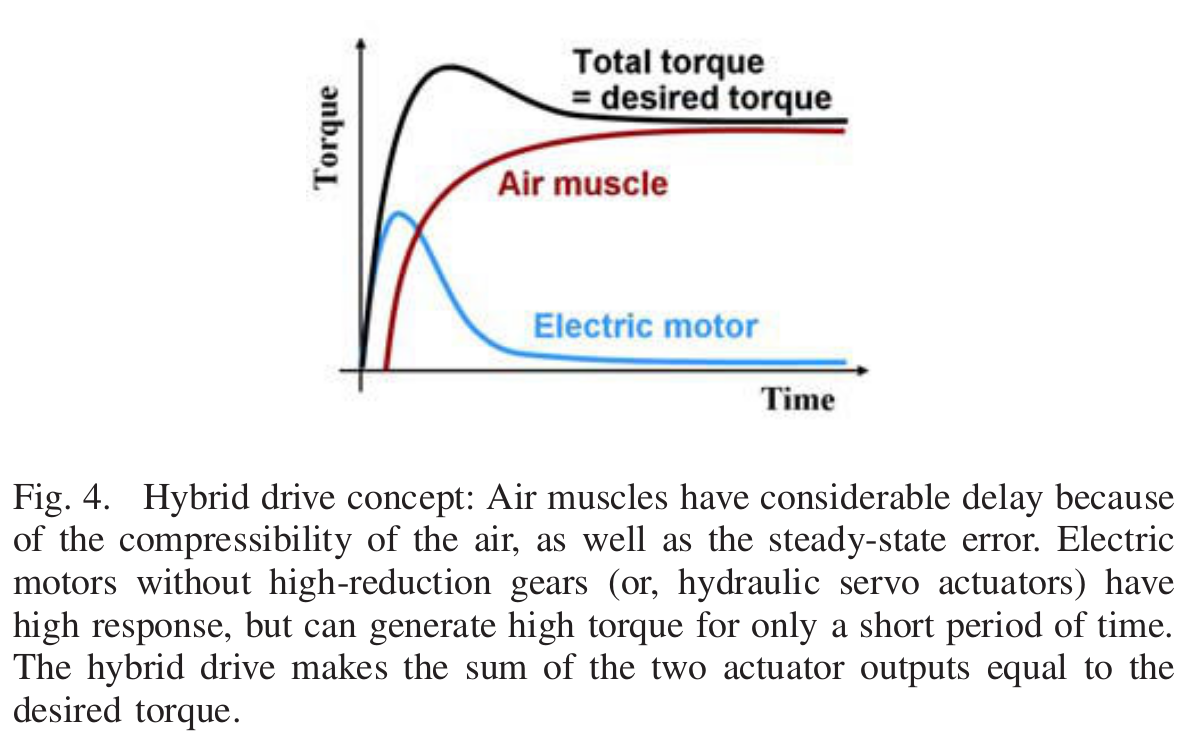
\includegraphics[width=3.5in]{exos/figs/xor_hybrid_drive_torque_time.png}
\end{figure}  

A challenge in using air muscles is that force reduces quadratically as a function of contraction.  For instance, at 30\% contraction, the force produced by FESTO rubber air muscles vanishes.  To address the issue, XoR's air muscles are strategically placed to generate forces in desired configurations.  

\begin{figure}[ht]
  \centering
  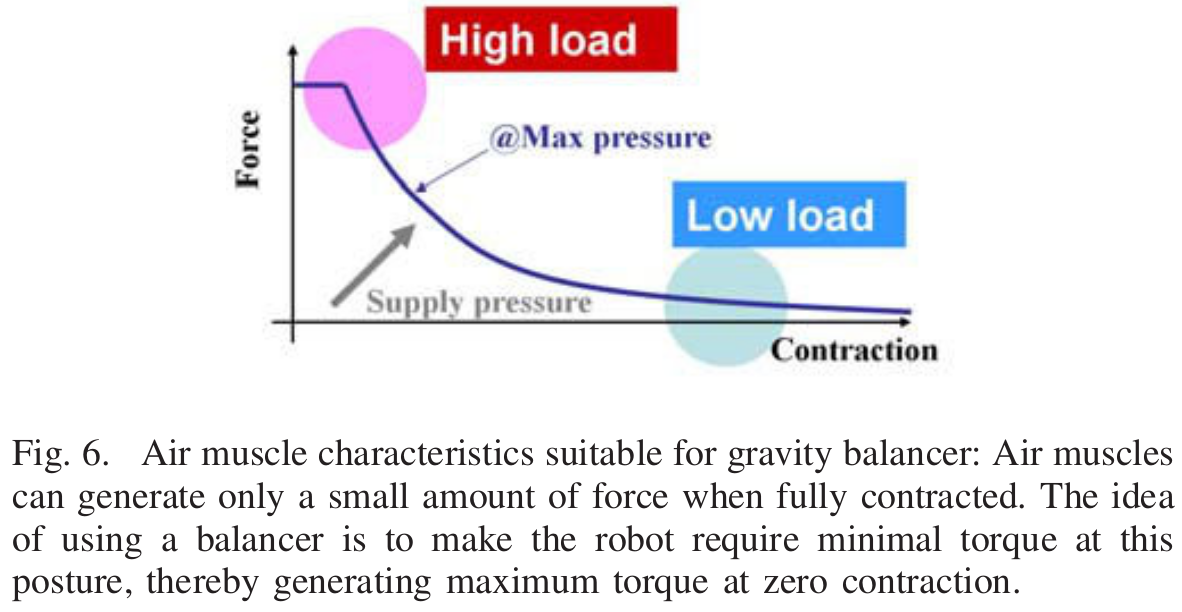
\includegraphics[width=3.5in]{exos/figs/xor_air_muscle_force_vs_contraction.png}
\end{figure}

In implementation, the XoR uses rubber air muscles (MDSP-40) connected to pulleys via tendons and to EP regulators in the backpack (a constant pressure and cam system is being tested to reduce weight required for backpack air valves).  The electric actuator is a geared, 200W brushless DC motor (Maxon EC powermax 30) rated at 4.7 A, which transmits power to joints through a belt and pulley system with a 57.5 gear ratio. The motor is backdrivable with 0.12 Nm output torque and up to 34.5 Nm (for short duration) at every joint.  The design yields a relatively high range of motion (up to 120 degrees) with a 150 Nm load capacity.  However, experiments reveal the need for bi-directional pneumatic actuation at hip joints.

For sensing, XoR is equipped with \textbf{rotary encoders} at joints, an \textbf{IMU} in the backpack, \textbf{load cells} in the feet, and is networked to servers capable of providing \textbf{EMG}, NIRS, and EEG data.  A control PC running at 1 KHz, pulse counter, amplifiers, Digital IO are external and so not included in the weight of the unit.  Human operators are outfitted with a \textbf{goniometer}.


\subsubsection{Control}

The XoR control strategy applied in \cite{XoRkinemExtraction2012} has two main components.  First, a proportional-derivative (PD) feedback controller tracks desired joint angles and angular velocities that correspond to the state of the exoskeleton required to assist the human operator.  To obtain this state (specifying the desired joint angles / velocities), the controller simultaneously measures the joint angle trajectories of the human user (goniometer) and of the robot (encoders), and uses canonical correlation analysis (CCA) to extract latent variables in the kinematic relationship between the two.

\begin{figure}[ht]
  \centering
  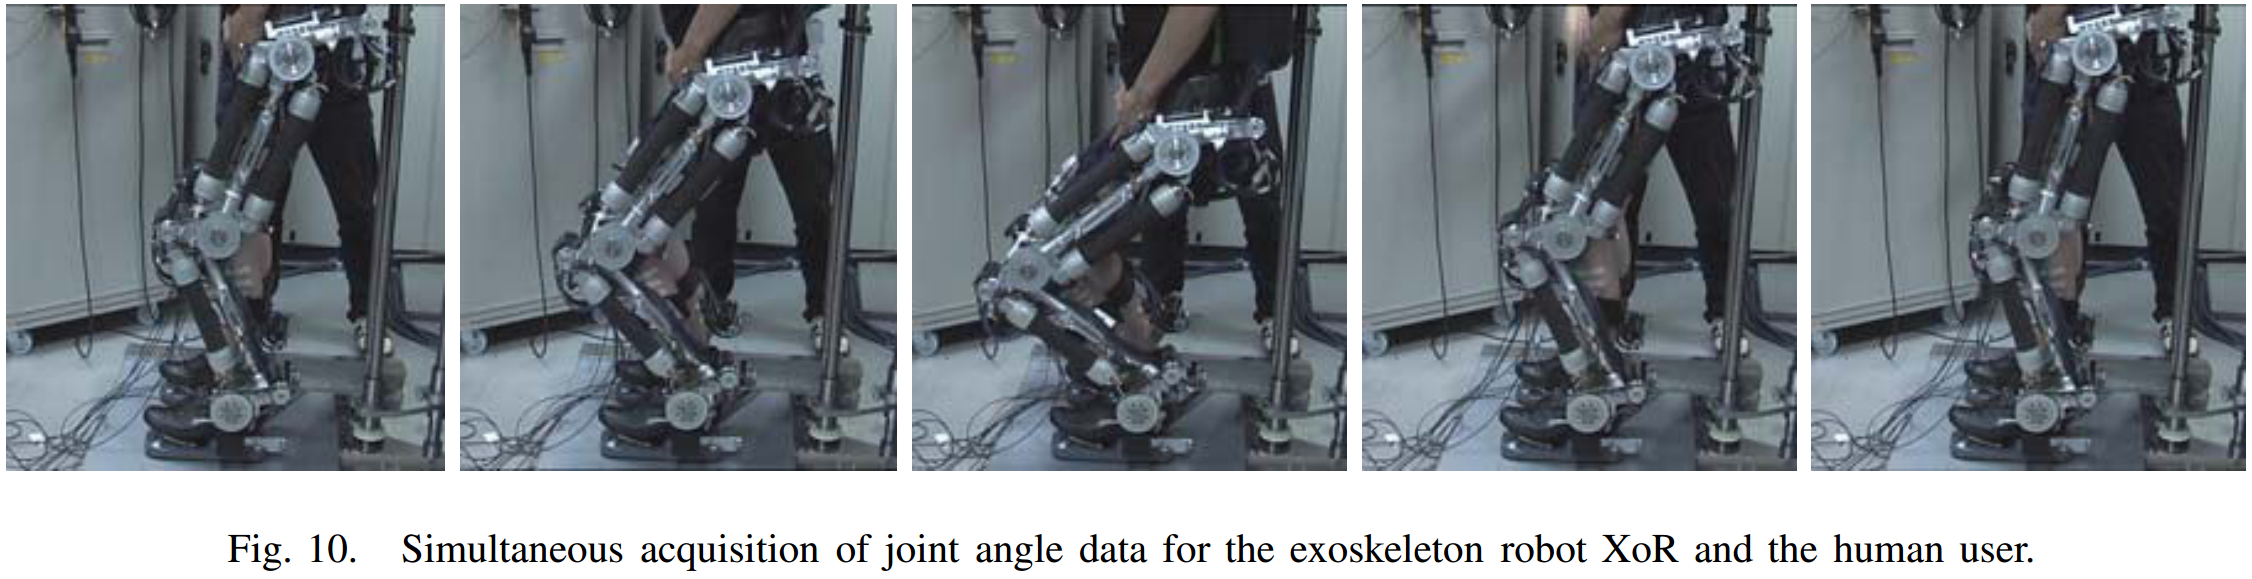
\includegraphics[width=6.0in]{exos/figs/xor_joint_angles.png}
\end{figure}

To avoid relying on high gain feedback, XoR incorporates user intent through EMG data.  The controller rectifies and low pass filters (10 Hz cut-off) data measured in the pilot's quadriceps femoris, tensor fasciae latate, gluteus medius, and tibialis anterior. 
It sets desired joint angles and velocities, ${\bf x} = ({\bf \theta}, \dot{\bf \theta})$, from the EMG data, ${\bf u} = (EMG_1 \dots EMG_n)$, using a linear prediction model, 
\[{\bf x}(k+1) = \mA{\bf x}(k)+\mB{\bf u}(k),\].  
The controller uses the angular measurements required to perform CCA and EMG data to derive the model's $\mA$ and $\mB$ terms.  The predicted state from EMG model provides the desired input to yet another PD controller: 
\[\tau_i = K_p (\theta_i^d - \theta_i) + K_d (\dot\theta_i^d - \dot \theta_i),\] 
with gains of $K_p = 1000$ and $K_d = 100$.

In hip tracking experiments, the team found EMG data to be helpful.  When using EMG signals, XoR achieved a mean squared error of $1.8E^{-3}$.  Without the EMG data, the mean squared error increased to $2.1$.  Additional experiments confirm the air muscles can effectively perform gravity compensation when used in conjunction with electric actuators (to correct for torque errors induced by inaccuracies in the model mapping position to toque in air muscles).


\subsection{Assessment and Recommendations}

The XoR prototype uses a promising hybrid actuation scheme to achieve both fast peak torque response and higher sustained torque while remaining lightweight.  It tracks human motion with feedback from a goniometer and feedforward control provided by EMG data.  These human intention / sensing modalities are both difficult to implement due to noise and calibration issues.  However, capturing the user intent is important, especially in the presence of external disturbances.  If the sensory system were improved (e.g, wearable ``robot skin'' sensing arrays), this exoskeleton design could be highly effective. 

\nocite{*}
\printbibliography[heading=subbibliography]

The figures in this section were obtained from \cite{xorDesign2011,XoRkinemExtraction2012}. Materials presented are based on the references above.

\end{refsection}